\subsection{Definition of a quiver}

DEFINITION 1. --- A quiver is a quadruple (S, F, o, t), where S and F are sets and o, t are maps from F to S.

Let \(C = (S, F, o, t)\) be a quiver. The elements of S are called the vertices of C. The elements of F are called the arrows of C. Let f be an arrow of C; the vertex \(o(f)\) is called the origin or source of f, the vertex \(t(f)\) is called the term, or the target of f; one also says that f connects the vertex \(o(f)\) to the vertex \(t(f)\) . The maps o and t are called respectively the source and target maps, or origin and term, of the quiver C.

When C is a quiver, \(\operatorname{Som}(\mathrm{C})\) , \(\operatorname{Fl}(\mathrm{C})\) \(o_{C}\) and \(t_{C}\) will denote respectively the set of vertices, that of arrows, the source map, and the target map of C. Let a and b be vertices of C; the set of arrows of C joining a to b is denoted \(\operatorname{Fl}_{a,b}(\mathrm{C})\) , or equivalently \(C_{a,b}\) .

To facilitate understanding of the reasoning, one may represent a quiver by a drawing composed of points and arrowed lines corresponding respectively to the vertices and to the arrows. The drawing:

\pandocbounded{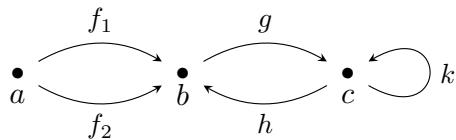
\includegraphics[keepaspectratio]{images/part001_552ae758.jpg}}

represents a quiver whose vertices are a, b, c, and whose arrows are \(f_{1}, f_{2}, g, h, k\) and the source and target maps are given by

\[
\begin{array}{c c c c} o (f _ {1}) = o (f _ {2}) = a & \quad o (g) = b & \quad o (h) = c & \quad o (k) = c \\ t (f _ {1}) = t (f _ {2}) = b & \quad t (g) = c & \quad t (h) = b & \quad t (k) = c. \end{array}
\]

